\documentclass{article}
\usepackage[utf8]{inputenc}
\usepackage{amsmath, amssymb, graphicx}
\usepackage[colorlinks=false, hidelinks]{hyperref}
\usepackage{listings}
\usepackage{xcolor}
\usepackage{graphicx}
\usepackage[english]{babel}
\usepackage{multirow}
\usepackage{booktabs}  % For \toprule, \midrule, \bottomrule in tables
\usepackage{float}     % For better positioning control with [H]
\usepackage{csquotes}

\usepackage{chngcntr}
\counterwithin{figure}{section}
\counterwithin{table}{section}

% For long mathematical formulas
\usepackage{mathtools}

% To help with overflows
\emergencystretch=1em
\setlength{\parindent}{15pt}

% To replace all position labels h with H
\makeatletter
\renewcommand{\fps@figure}{H}
\renewcommand{\fps@table}{H}
\makeatother

% Reference package - modify these lines
\usepackage[
    backend=biber,
    style=apa,
    sorting=nyt,
    giveninits=true,
    uniquename=init,
    natbib=true
]{biblatex}
\addbibresource{main.bib}

% This is to set all reference as a hyperlink
\DeclareFieldFormat{bibhyperrefnonest}{%
  \DeclareFieldFormat{bibhyperref}{##1}%
  \bibhyperref{#1}}

\DeclareCiteCommand{\parencite}[\mkbibparens]
  {\usebibmacro{cite:init}%
   \usebibmacro{prenote}}
  {\usebibmacro{citeindex}%
   \printtext[bibhyperrefnonest]{\usebibmacro{cite}}}
  {}
  {\usebibmacro{postnote}%
   \usebibmacro{cite:post}}

\lstdefinestyle{promptstyle}{
    basicstyle=\small\ttfamily,
    breaklines=true,
    frame=single,
    captionpos=b,
    keepspaces=true,
    numbers=none,
    showstringspaces=false,
    breakatwhitespace=false
}

\title{Machine Learning-based Control Techniques versus Traditional PID Controllers}
\author{Marcos Soto \\ \textit{Loyola Andalusia University}}
\date{}

\begin{document}

\maketitle

\begin{abstract}
  In the process industry, PID (Proportional, Integral, Derivative) controllers have historically been the dominant tool for valve control 
  due to their simplicity and robustness. However, their performance is compromised in multivariable, nonlinear systems subject to disturbances, such as in well testing 
  \parencite{song_dynamic_2023} and other complex industrial operations. This work presents a systematic review (2015–2025), following PRISMA methodology and PICO formulation, comparing 
  machine learning (ML)-based techniques including artificial neural networks (ANN), adaptive control and reinforcement learning (RL), with traditional PID controllers. 
  The databases Web of Science, Scopus and Google Scholar were consulted, identifying 97 initial records and selecting 7 relevant studies after applying 
  inclusion criteria. Results indicate that ANN and hybrid Neuro-PID techniques reduce overshoot and settling time by 15–40\% compared to manually tuned PIDs, 
  while adaptive approaches such as CLOE+RST maintain stability in multiple valves without re-tuning. RL showed operational resilience in 
  sensor failure scenarios and inference times <5 ms, compatible with real-time control. Successful implementations in PLC, FPGA and SCADA environments are documented, supporting 
  industrial viability. Although no cases of LLMs applied directly to valve control were found, opportunities for their use as supervisory agents 
  and autonomous tuning are identified. It is concluded that ML techniques offer significant advantages over PID in complex industrial environments and that their extrapolation to well testing 
  represents an applied research opportunity.
\end{abstract}

\section{Introduction}

In the process industry, PID (Proportional Integral Derivative) controllers have been the predominant solution for regulating variables due to their simplicity and robustness.
However, their performance is limited in complex conditions: multivariable systems, for example well testing separators where they must control multiple valves 
that are part of the same process, under strongly nonlinear conditions, with noise, disturbances or changing dynamics requiring frequent re-tuning and may exceed 
their optimal capabilities. Therefore, interest has grown in the use of control techniques based on neural networks and machine learning, which promise to adapt better to these 
complexities than traditional PIDs. \parencite{cabrera-rufino_implementation_2022} The central objective is to evaluate whether such intelligent approaches can improve process valve control in well 
testing (well testing) \parencite{song_dynamic_2023} compared to conventional PID controllers. In addition, analogous studies in other industries are explored to extract applicable ideas and 
cutting-edge strategies (including LLM language models) oriented towards autonomous systems with minimal human intervention are considered. The following presents a 
state-of-the-art review in this regard, emphasizing conceptual work and theoretical designs that will serve as a basis for subsequent experimentation.

\section{Methodology}

\subsection{Search strategies}

A systematic search was conducted in the databases: Web of Science (WoS), Scopus, Google Scholar. \parencite{liberati_prisma_2009}

The search terms used combine keywords about control techniques and application domain:

\begin{itemize}
  \item "machine learning" AND "valve control"
  \item "PID" AND "neural networks" AND "industrial process"
  \item "reinforcement learning" AND "control valves"
  \item "LLM" AND "valve control"
\end{itemize}


Filters were applied by year ($\geq$2015), language (English and Spanish), and document type (peer-reviewed articles, relevant conferences and technical gray literature).
The initial strategy sought to maximize retrieval and then refine by relevance.

\subsection{Research questions (PICO)}

\begin{itemize}
  \item \textbf{Population (P)}: Industrial processes with valve control (well testing, three-phase separation, refinery and analogous contexts).
  \item \textbf{Intervention (I)}: Machine learning-based control (neural networks, reinforcement learning, neuro-PID hybrids, LLMs/Agents).
  \item \textbf{Comparison (C)}: Traditional controllers (PID/PI), including variants and classical tuning.
  \item \textbf{Outcome (O)}: Control performance (overshoot, settling time, IAE/ISE, RMS error), robustness to disturbances/noise, autonomy (less human intervention), implementation feasibility (PLC/SCADA/real time).
\end{itemize}

\subsection{Main question}

In industrial process valve control (P), do ML-based techniques (I) outperform traditional PID controllers (C) in loop performance, robustness and autonomy (O)?

\subsubsection{Secondary questions}

\begin{itemize}
  \item When does ML replace PID and when does it complement it (hybrid)?
  \item What level of validation do they present (simulation, pilot, field)?
  \item How feasible is it to implement them in real industrial environments?
\end{itemize}

\subsubsection{Inclusion criteria}

\begin{itemize}
  \item Studies that implement or simulate valve control in industrial processes.
  \item Use of ML (neural networks, RL, neuro-PID hybrids, intelligent agents).
  \item Comparison with PID (direct or indirect).
  \item Clearly reported performance metrics.
  \item Applicability to real or simulated industrial environments (PLC, SCADA, embedded control).
\end{itemize}

\subsubsection{Exclusion criteria}

\begin{itemize}
  \item Exclusively theoretical works without valve control case.
  \item ML control studies without reference to PID or without quantitative metrics.
  \item Applications outside industrial processes.
\end{itemize}

\section{Results}

From the systematic searches in WoS, Scopus and Google Scholar, 97 initial records were obtained, after eliminating duplicates and applying the PICO inclusion criteria, 
7 studies were selected that compare machine learning (ML)-based control techniques, including artificial neural networks (ANN), adaptive control and 
reinforcement learning (RL), with classical PID or PI controllers, in industrial contexts of valve control or analogous operations.

% Add image
\begin{figure}[H]
  \centering
  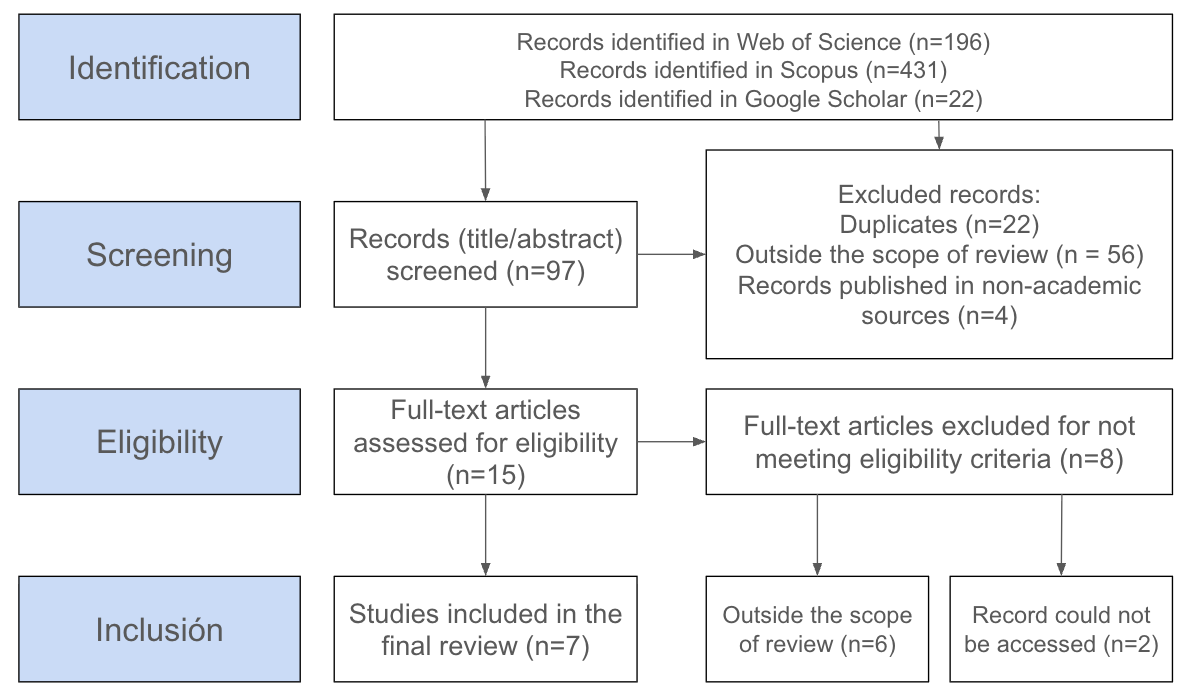
\includegraphics[width=0.8\textwidth]{img/prisma_chart.png}
  \caption{PRISMA diagram article selection}
  \label{fig:comparacion_ml_pid}
\end{figure}

\subsubsection{Context and applications}

\begin{itemize}
  \item High nonlinearity industrial processes: phase separation, butterfly valves, hot blast furnaces, flow and pressure control in thermal circuits.
  \item Transferability to well testing: at least 4 studies address valves and multivariable systems comparable in dynamics and complexity.
\end{itemize}

\subsubsection{Evaluated techniques}
\begin{itemize}
  \item ANN and hybrid neuro-PID: used to improve tuning and response to disturbances, reducing overshoot and settling time.
  \item Adaptive control (CLOE + RST): iterative closed-loop adaptation to compensate for variations between valves.
  \item Reinforcement learning (RL): DQN agents and variants with attention and recurrent networks, trained to make valve adjustment decisions in real time.
  \item Other approaches: neurofuzzy models and evolutionary algorithms as PID optimizers.
\end{itemize}

\subsubsection{Variables and metrics}

\begin{itemize}
  \item Controlled variables: pressure, temperature, flow rate, valve position.
  \item Comparative metrics: overshoot, settling time, RMSE, IAE/ISE, action precision, inference time, robustness to disturbances and sensor failures.
\end{itemize}

\subsubsection{Comparison with PID}

\begin{itemize}
  \item Quantitative improvements: in most cases, reduction of RMS error and settling time between 15\% and 40\% compared to manually tuned PID.
  \item Failure scenarios: in one RL case, the agent maintained stable operation despite loss of flow signal, while the PID/classical logic-based system could not operate.
  \item Robustness and adaptability: adaptive control achieved maintaining stability margins ($\Delta$M$\geq$0.5) in different valves without manual retuning.
\end{itemize}

\subsubsection{Validation}

\begin{itemize}
  \item 3 studies in real plant (RL in blast furnaces, ANN in thermal circuits, adaptive control in valve bench).
  \item 4 studies in simulation or pilot with detailed models, all replicable in industrial environments.
\end{itemize}

\subsubsection{Implementation feasibility}

\begin{itemize}
  \item Tools: MATLAB/Simulink, Python, embedded environments (Arduino, PLC, FPGA).
  \item Inference times reported in RL applications <5 ms, viable for real-time control.
\end{itemize}

\section{Discussion}

The systematic review identified seven studies (2015–2025) comparing machine learning (ML)-based controllers, primarily artificial neural networks (ANN), 
adaptive control and reinforcement learning (RL), with classical PID or PI in nonlinear industrial processes. Although the contexts include butterfly valves, hot blast 
furnaces, thermal systems and fluid circuits, clear patterns of relevance for well testing and valve control in three-phase separators are observed.

Performance improvements and adaptability

In most cases, ANN techniques and Neuro-PID hybrids showed quantitative improvements in overshoot, settling time and RMS/IAE error, with typical 
performance increases between 15\% and 40\% compared to manually tuned PID. The advantage of hybrids lies in maintaining the robustness and simplicity of PID while an ML module 
adjusts gains online to adapt to load or dynamic changes. This was especially effective in pneumatic actuators and servo-valves with friction, 
stiction or fluid compressibility.

Adaptive control and robustness

Adaptive control based on closed-loop identification (CLOE) and RST redesign stood out for its ability to compensate for variations between valves without the need for 
manual re-tuning, maintaining robust stability margins ($\Delta$M$\geq$0.5). This approach offers a pragmatic transition between classical PID and advanced ML techniques, with 
viable implementation on embedded hardware.

Reinforcement learning and operational autonomy

RL, although less widespread in real industrial environments, showed very promising results: in one case, a DQN agent with attention architecture deployed in plant 
maintained stable control even in the face of critical sensor failures (flow meters), surpassing previous PID/expert logic. This type of resilience aligns with the goal of 
minimal human intervention and opens the door to autonomous systems.

Industrial viability and limitations

Several studies demonstrated that ML solutions can be implemented in PLC, FPGA and SCADA environments without compromising latency. In RL cases, the inference times 
reported (<5 ms) were compatible with real-time control. However, most implementations are still limited to pilot environments or advanced simulations, and 
adoption in production is conditioned by the need for large volumes of data and extensive validation.

Projection towards emerging technologies

Although no direct implementations of large language models (LLM) in valve control were found, their potential as supervisory agents, control loop coordinators 
and autonomous diagnostics is evident. Integrating LLM with ML controllers could enable supervisory systems capable of adjusting parameters, coordinating strategies 
and responding to failures without human intervention.


\section{Conclusions}

Superiority of ML techniques over PID

The evidence collected in seven studies demonstrates that ANN, adaptive control and RL outperform classical PID in industrial scenarios characterized by nonlinearity, 
coupling and changing operating conditions. Quantitative improvements in overshoot, settling time and RMS/IAE error support their adoption as alternatives 
or complements to conventional controllers.

Advantage of hybrid and adaptive approaches

Solutions such as Neuro-PID or adaptive control CLOE + RST offer a balance between the robustness and simplicity of PID and the online adjustment capability of ML, 
being especially effective in actuators with friction, stiction or mechanical variability.

RL and operational resilience

Real plant validation of RL agents with inference times below 5 ms demonstrates viability for real-time control. Their ability to maintain 
stable operation in the face of critical sensor failures confirms the potential of RL to achieve more autonomous and fault-tolerant systems.

Technological viability in industrial environments

The successful implementation of these techniques in PLC, FPGA and SCADA systems confirms that latency and processing limitations do not constitute an insurmountable technical barrier 
, although the transition to large-scale continuous operation remains a challenge.

Future opportunities in well testing

Although no specific cases of ML applied to valve control in three-phase well testing separators were found, the extrapolation of techniques validated in 
analogous industries is feasible. This gap opens the opportunity to design controlled experiments that reproduce real well testing conditions to validate these approaches.

Integration with emerging technologies

LLMs, although not yet applied to valve control, are emerging as promising tools for supervision, coordination of multiple loops and autonomous adjustment 
of parameters, complementing the adaptive capabilities of ML controllers.


\section{References}
% Include your references using BibTeX
\printbibliography

\end{document}